\documentclass[a4paper]{article}

%\renewcommand*{\sectfont}{\normalfont\bfseries}

\usepackage{fixltx2e}
\usepackage{isomath}

\usepackage[utf8]{inputenc}
\usepackage[T1]{fontenc}
\usepackage[british]{babel}

\makeatletter
\useshorthands{"}%
\defineshorthand{"-}{\nobreak-\bbl@allowhyphens}
\defineshorthand{"=}{\nobreak--\bbl@allowhyphens}
\makeatother

\usepackage{amsmath}
\usepackage{amsfonts}
\usepackage{natbib}
\usepackage{proof}
\usepackage{tikz}

\usepackage{microtype}

\newcommand*{\INFER}[3][]{\ensuremath{\infer[\text{\footnotesize #1}]{\mathstrut #2}{\mathstrut #3}}}

\newcommand*{\GRAPHR}[2]{%
	\begin{tikzpicture}[xscale=0.5, yscale=0.5]
		\path[draw, white] (0, 0) rectangle (1, 1);
		\path[thick, ->] (0, 0) edge[out=90, in=90, looseness=3] (1, 0);
		\node[anchor=north] at (0, 0) {$\mathstrut #1$};
		\node[anchor=north] at (1, 0) {$\mathstrut #2$};
	\end{tikzpicture}%
}

\newcommand*{\GRAPHL}[2]{%
	\begin{tikzpicture}[xscale=0.5, yscale=0.5]
		\path[draw, white] (0, 0) rectangle (1, 1);
		\path[thick, <-] (0, 0) edge[out=90, in=90, looseness=3] (1, 0);
		\node[anchor=north] at (0, 0) {$\mathstrut #1$};
		\node[anchor=north] at (1, 0) {$\mathstrut #2$};
	\end{tikzpicture}%
}

\newcommand*{\GRAPHH}[2]{%
	\begin{tikzpicture}[xscale=0.5, yscale=0.5]
		\path[draw, white] (0, 0) rectangle (1, 1);
		\draw[thick, help lines] (0, 0) rectangle (1, 0.75);
		\node[anchor=north] at (0, 0) {$\mathstrut #1$};
		\node[anchor=north] at (1, 0) {$\mathstrut #2$};
	\end{tikzpicture}%
}

\newcommand*{\SEQR}[2]{%
	\begin{tikzpicture}[xscale=0.5, yscale=0.5]
		\path[draw, white] (0, 0) rectangle (3.5, 1);
		\path[thick, ->] (0, 0) edge[out=90, in=90, looseness=3] (1, 0);
		\path[thick, ->] (2.5, 0) edge[out=90, in=90, looseness=3] (3.5, 0);
		\node at (1.75, 0.5) {$\mathstrut\cdots$};
		\node[anchor=north] at (0, 0) {$\mathstrut #1$};
		\node[anchor=north] at (3.5, 0) {$\mathstrut #2$};
	\end{tikzpicture}%
}

\newcommand*{\SEQL}[2]{%
	\begin{tikzpicture}[xscale=0.5, yscale=0.5]
		\path[draw, white] (0, 0) rectangle (3.5, 1);
		\path[thick, <-] (0, 0) edge[out=90, in=90, looseness=3] (1, 0);
		\path[thick, <-] (2.5, 0) edge[out=90, in=90, looseness=3] (3.5, 0);
		\node at (1.75, 0.5) {$\mathstrut\cdots$};
		\node[anchor=north] at (0, 0) {$\mathstrut #1$};
		\node[anchor=north] at (3.5, 0) {$\mathstrut #2$};
	\end{tikzpicture}%
}

\newcommand*{\SEQM}[2]{%
	\begin{tikzpicture}[xscale=0.5, yscale=0.5]
		\path[draw, white] (0, 0) rectangle (3.5, 1);
		\path[thick] (0, 0) edge[out=90, in=90, looseness=3] (1, 0);
		\path[thick] (2.5, 0) edge[out=90, in=90, looseness=3] (3.5, 0);
		\node at (1.75, 0.5) {$\mathstrut\cdots$};
		\node[anchor=north] at (0, 0) {$\mathstrut #1$};
		\node[anchor=north] at (3.5, 0) {$\mathstrut #2$};
	\end{tikzpicture}%
}

\newcommand*{\SEQU}[2]{%
	\begin{tikzpicture}[xscale=0.5, yscale=0.5]
		\path[draw, white] (0, 0) rectangle (3.5, 1);
		\path[thick] (0, 0) edge[out=90, in=90, looseness=3] (1, 0);
		\path[thick] (2.5, 0) edge[out=90, in=90, looseness=3] (3.5, 0);
		\node at (1.75, 0.5) {$\mathstrut\cdots$};
		\node at (1.75, 0.5) {$//$};
		\node[anchor=north] at (0, 0) {$\mathstrut #1$};
		\node[anchor=north] at (3.5, 0) {$\mathstrut #2$};
	\end{tikzpicture}%
}

\linespread{1.1}

\newcommand*{\ALGEBRA}[1]{\mathfrak{#1}}
\newcommand*{\FUN}[1]{\text{#1}}
\newcommand*{\SET}[1]{\{#1\}}
\newcommand*{\SETC}[2]{\SET{\,#1\mid #2\,}}
\newcommand*{\TERMS}[1]{T({#1})}

\begin{document}

\title{Tabulation of Noncrossing Acyclic Digraphs}

\author{%
	Marco Kuhlmann\\
	Department of Computer and Information Science\\
	Linköping University, Sweden}

\maketitle


\section{Introduction}

A \emph{noncrossing graph} of size $n$ is a graph drawn on $n$ (labelled) vertices on a circle such that the edges are straight"-line segments that do not cross.
Here we are concerned with \emph{noncrossing acyclic digraphs}.
Examples of such structures are given in Figure~\ref{fig:ncdags-examples}.

\begin{figure}
	\centering\footnotesize
	\input ncdags-examples
	\caption{Some (out of 335) noncrossing acyclic digraphs of size~4.}
	\label{fig:ncdags-examples}
\end{figure}

In this note we present a tabulation method for noncrossing acyclic digraphs:
We specify an algorithm that produces a compact (polynomial"-space) representation of the set of all noncrossing acyclic digraphs of a given size~$n$.
Let this set be denoted by $\mathcal{N}_n$.
We provide an algebra $\ALGEBRA{A}$ and show how to construct, for a given size~$n$, a regular tree grammar~$G_n$ \citep{comon2008tree} such that
\begin{displaymath}
	\mathcal{N}_n = \SETC{\FUN{val}_{\ALGEBRA{A}}(t)}{t \in L(G_n)}\,,
\end{displaymath}
where $\FUN{val}_{\ALGEBRA{A}}(t)$ denotes the value of the term~$t$ in the algebra~$\ALGEBRA{A}$.
That is, the terms generated by $G_n$ are exactly `derivation trees' for the graphs in~$\mathcal{N}_n$.
Moreover, our construction is such that the valuation is injective when restricted to $L(G_n)$, meaning that every graph in $\mathcal{N}_n$ has a \emph{unique} derivation tree.

\iffalse

\begin{center}
	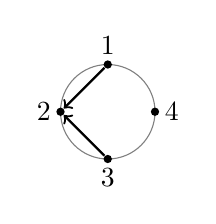
\begin{tikzpicture}[scale=0.6]
		\draw[gray] (0, 0) circle (1);
		\node[fill,circle,inner sep=0pt,minimum size=3pt] (c1) at (0, 1) {};
		\node[fill,circle,inner sep=0pt,minimum size=3pt] (c2) at (-1, 0) {};
		\node[fill,circle,inner sep=0pt,minimum size=3pt] (c3) at (0, -1) {};
		\node[fill,circle,inner sep=0pt,minimum size=3pt] (c4) at (1, 0) {};
		\node[anchor=south] at (c1) {$1$};
		\node[anchor=east] at (c2) {$2$};
		\node[anchor=north] at (c3) {$3$};
		\node[anchor=west] at (c4) {$4$};
		\draw[thick,->] (c1) -- (c2);
		\draw[thick,->] (c3) -- (c2);
	\end{tikzpicture}
\end{center}

\fi


\section{Algebraic Structure}

Our tabulation is based on a certain algebraic structure for noncrossing digraphs.
To present this structure, we recall some standard terminology:
A \emph{signature} is a set~$\Sigma$ of function symbols~$f$, each of which has been assigned a non"-negative integer called its \emph{rank}.
Given a signature~$\Sigma$, the set of \emph{terms} over~$\Sigma$, denoted by $\TERMS{\Sigma}$, is defined as the smallest set $T \subseteq \Sigma^*$ such that $f t_1 \cdots t_m \in T$ whenever $f$ is a function symbol from~$\Sigma$ with rank~$m$ and $t_1, \dots, t_m \in T$.
Note that we write terms as strings; however, we also use the familiar notation with parentheses and commas.
An \emph{algebra}~$\ALGEBRA{A}$ consists of a non"-empty set~$A$ called the \emph{domain} of~$\ALGEBRA{A}$ and, for each symbol $f \in \Sigma$ with rank~$m$, a total function $f^{\ALGEBRA{A}}\mathpunct{:}\ A^m \to A$, the \emph{operation} associated with~$f$.
The \emph{value} of a term $t \in \TERMS{\Sigma}$ in~$\ALGEBRA{A}$, denoted by $\FUN{val}_{\ALGEBRA{A}}(t)$, is defined recursively as
\begin{displaymath}
	\FUN{val}_{\ALGEBRA{A}}(f t_1 \cdots t_m)
	=
	f^{\ALGEBRA{A}}(\FUN{val}_{\ALGEBRA{A}}(t_1), \dots, \FUN{val}_{\ALGEBRA{A}}(t_m))\,.
\end{displaymath}
consists of a single constant and three operations.
The constant, which we shall denote by~$c$, is the graph with two nodes and no edges.
The three operations are:
\begin{itemize}
	\item $\FUN{ext}_{\rightarrow}(G)$: Extend a given graph $G$ by adding an edge $1 \to n$.
	\item $\FUN{ext}_{\leftarrow}(G)$: Extend a given graph $G$ by adding an edge $n \to 1$.
	\item $\FUN{conc}(G_1, G_2)$: Concatenate two graphs~$G_1$ and~$G_2$, identifying vertex $n$ of $G_1$ with vertex $1$ of $G_2$.
\end{itemize}

\begin{displaymath}
	\FUN{ext}_{\rightarrow}(\GRAPHH{1}{2}) = \GRAPHR{1}{2}
\end{displaymath}

For example, there are 3 noncrossing acyclic digraphs on 2 of size 2: the graph with the edge $1 \to 2$, the graph with the edge $2 \to 1$, and the graph with no edges.


\section{Inference System}

We specify our algorithm in terms of a deduction system \citep{shieber1995principles}.
We assume that we are given a number $n \geq 2$.

\subsection{Items}

A noncrossing acyclic digraph is called \emph{edge"-covered} if there an edge between its extremal vertices.
We use the following items to represent edge"-covered graphs where the covering edge is $i \to j$ or $j \to i$, respectively:
\begin{displaymath}
	\GRAPHR{i}{j}
	\qquad
	\GRAPHL{i}{j}
\end{displaymath}

If a graph is not edge"-covered, we distinguish two cases, depending on whether the graph is weakly connected, that is, whether there exists an path between the extremal vertices.
If the graph is weakly connected, we additionally distinguish three cases:
\begin{enumerate}
	\item There is a directed path from the leftmost vertex to the rightmost vertex.
	\item There is a directed path from the rightmost vertex to the leftmost vertex.
	\item There is no directed path between the two extremal vertices.
\end{enumerate}
We use the following 
\begin{displaymath}
	\SEQR{i}{j}
	\qquad
	\SEQL{i}{j}
	\qquad
	\SEQM{i}{j}
\end{displaymath}
Finally, if the graph is not weakly connected, we distinguish two cases, depending on whether the graph is of size~$2$ (in which case it consists of two nodes and no edges) or of size greater than~$2$.
\begin{displaymath}
	\GRAPHH{i}{j}
	\qquad
	\SEQU{i}{j}
\end{displaymath}

, depending on whether there exists the path between the extremal vertices consists of 

Either there exists 

\begin{enumerate}
	\item Is the graph edge"-covered or not?
	\item If the graph is edge"-covered, does the cover edge point rightward (from vertex~$1$ to vertex~$n$) or leftward (from vertex~$n$ to vertex~$1$)?
	\item If the graph is not edge"-covered, is it weakly connected or not?
	\item If the graph is not edge"-covered but weakly connected, are the extremal vertices connected by a rightward directed path (from vertex~$1$ to vertex~$n$) or a leftward directed path (from vertex~$n$ to vertex~$1$) or only an undirected path?
\end{enumerate}
The \emph{items} of our logic take one of six possible forms.

\begin{displaymath}
	\GRAPHR{i}{j}
	\qquad
	\GRAPHL{i}{j}
	\qquad
	\GRAPHH{i}{j}
\end{displaymath}
These items represent a noncrossing acyclic digraph whose leftmost node is $i$, whose rightmost node is $j$, and that has an edge $i \to j$ (first type) or $j \to i$.

\paragraph{Sequences}

The next three item types represent 

\paragraph{Unconnected}

\begin{displaymath}
	\SEQU{i}{j}
\end{displaymath}

\subsection{Axioms}

The axioms of our deduction systems are all items of the form
\begin{displaymath}
	\SEQU{i}{i + 1}
\end{displaymath}

\subsection{Rules}

We now present the rules of our deduction system.

\paragraph{Concatenate two edge"-covered graphs}

The first four rules simulate the concatenation of two edge"-covered graphs.
The result of such a concatenation is not edge"-covered but connected:
\begin{displaymath}
	\INFER{\SEQR{i}{k}}{\GRAPHR{i}{j} & \GRAPHR{j}{k}}
	\qquad
	\INFER{\SEQL{i}{k}}{\GRAPHL{i}{j} & \GRAPHL{j}{k}}
	\qquad
	\INFER{\SEQM{i}{k}}{\GRAPHR{i}{j} & \GRAPHL{j}{k}}
	\qquad
	\INFER{\SEQM{i}{k}}{\GRAPHL{i}{j} & \GRAPHR{j}{k}}
\end{displaymath}

\paragraph{Concatenate an edge"-covered graph and the elementary graph}

The next rules simulate the concatenation of an edge"-covered graph and the elementary graph.
The result of such a concatenation is neither edge"-covered nor connected.
There are four cases:
\begin{displaymath}
	\INFER{\SEQU{i}{k}}{\GRAPHR{i}{j} & \GRAPHH{j}{k}}
	\qquad
	\INFER{\SEQU{i}{k}}{\GRAPHH{i}{j} & \GRAPHR{j}{k}}
	\qquad
	\INFER{\SEQU{i}{k}}{\GRAPHL{i}{j} & \GRAPHH{j}{k}}
	\qquad
	\INFER{\SEQU{i}{k}}{\GRAPHH{i}{j} & \GRAPHL{j}{k}}
\end{displaymath}

\paragraph{Concatenate a connected graph and an edge"-covered graph}

The following rules simulate the concatenation of a connected graph and an edge"-covered graph.
The result of such a concatenation is not edge"-covered but connected.
There are 6 cases; we group these cases based on the type of the first argument of the concatenation operation.

\begin{trivlist}
	\item\relax \textit{Group~1: The first argument is R"-connected}
	\begin{displaymath}
		\INFER{\SEQR{i}{k}}{\SEQR{i}{j} & \GRAPHR{j}{k}}
		\qquad
		\INFER{\SEQM{i}{k}}{\SEQR{i}{j} & \GRAPHL{j}{k}}
	\end{displaymath}
	
	\item\relax \textit{Group~2: The first argument is L"-connected}
	\begin{displaymath}
		\INFER{\SEQM{i}{k}}{\SEQL{i}{j} & \GRAPHR{j}{k}}
		\qquad
		\INFER{\SEQL{i}{k}}{\SEQL{i}{j} & \GRAPHL{j}{k}}
	\end{displaymath}
	
	\item\relax \textit{Group~3: The first argument is neither R"-connected nor L"-connected}
	\begin{displaymath}
		\INFER{\SEQM{i}{k}}{\SEQM{i}{j} & \GRAPHR{j}{k}}
		\qquad
		\INFER{\SEQM{i}{k}}{\SEQM{i}{j} & \GRAPHL{j}{k}}
	\end{displaymath}
\end{trivlist}

\paragraph{Concatenate a connected graph and the elementary graph}

The next rules simulate the concatenation of a connected graph and the elementary graph.
The result of such a concatenation is an unconnected graph.
There are 3~cases:
\begin{displaymath}
	\INFER{\SEQU{i}{k}}{\SEQR{i}{j} & \GRAPHH{j}{k}}
	\qquad
	\INFER{\SEQU{i}{k}}{\SEQL{i}{j} & \GRAPHH{j}{k}}
	\qquad
	\INFER{\SEQU{i}{k}}{\SEQM{i}{j} & \GRAPHH{j}{k}}
\end{displaymath}

\paragraph{Concatenate aan unconnected graph and}

The next rules simulate the concatenation to an unconnected graph.
The result of such a concatenation is another unconnected graph.
There are 3~cases:
\begin{displaymath}
	\INFER{\SEQU{i}{k}}{\SEQU{i}{j} & \GRAPHR{j}{k}}
	\qquad
	\INFER{\SEQU{i}{k}}{\SEQU{i}{j} & \GRAPHL{j}{k}}
	\qquad
	\INFER{\SEQU{i}{k}}{\SEQU{i}{j} & \GRAPHH{j}{k}}
\end{displaymath}


\paragraph{Covering a graph}

The rules in the final group simulate the covering operation.
The result of such an operation is an edge"-covered graph.
There are 6~cases; we group them based on the direction of the covering edge.
\begin{trivlist}
	\item\relax \textit{Group~1: The covering edge is left"-to"-right}
	\begin{displaymath}
		\INFER[R99]{\GRAPHR{i}{j}}{\SEQR{i}{j}}
		\qquad
		\INFER{\GRAPHR{i}{j}}{\SEQM{i}{j}}
		\qquad
		\INFER{\GRAPHR{i}{j}}{\SEQU{i}{j}}
	\end{displaymath}
	
	\item\relax \textit{Group~2: The covering edge is right"-to"-left}
	\begin{displaymath}
		\INFER{\GRAPHL{i}{j}}{\SEQL{i}{j}}
		\qquad
		\INFER{\GRAPHL{i}{j}}{\SEQM{i}{j}}
		\qquad
		\INFER{\GRAPHL{i}{j}}{\SEQU{i}{j}}
	\end{displaymath}
\end{trivlist}

\section{Code}

The inference system can be implemented using a bottom-up dynamic programming algorithm.
The code is available on GitHub.


\section{Conclusion}

can be used to compute highest-scoring graph under an arc-factored scoring model, count the number of graphs, compute inside and outside scores


\bibliographystyle{plainnat}
\bibliography{mcqm}

\end{document}
